\documentclass[border=4pt]{standalone}
\usepackage{tikz}
\usetikzlibrary{positioning, arrows.meta, fit, backgrounds}

\begin{document}
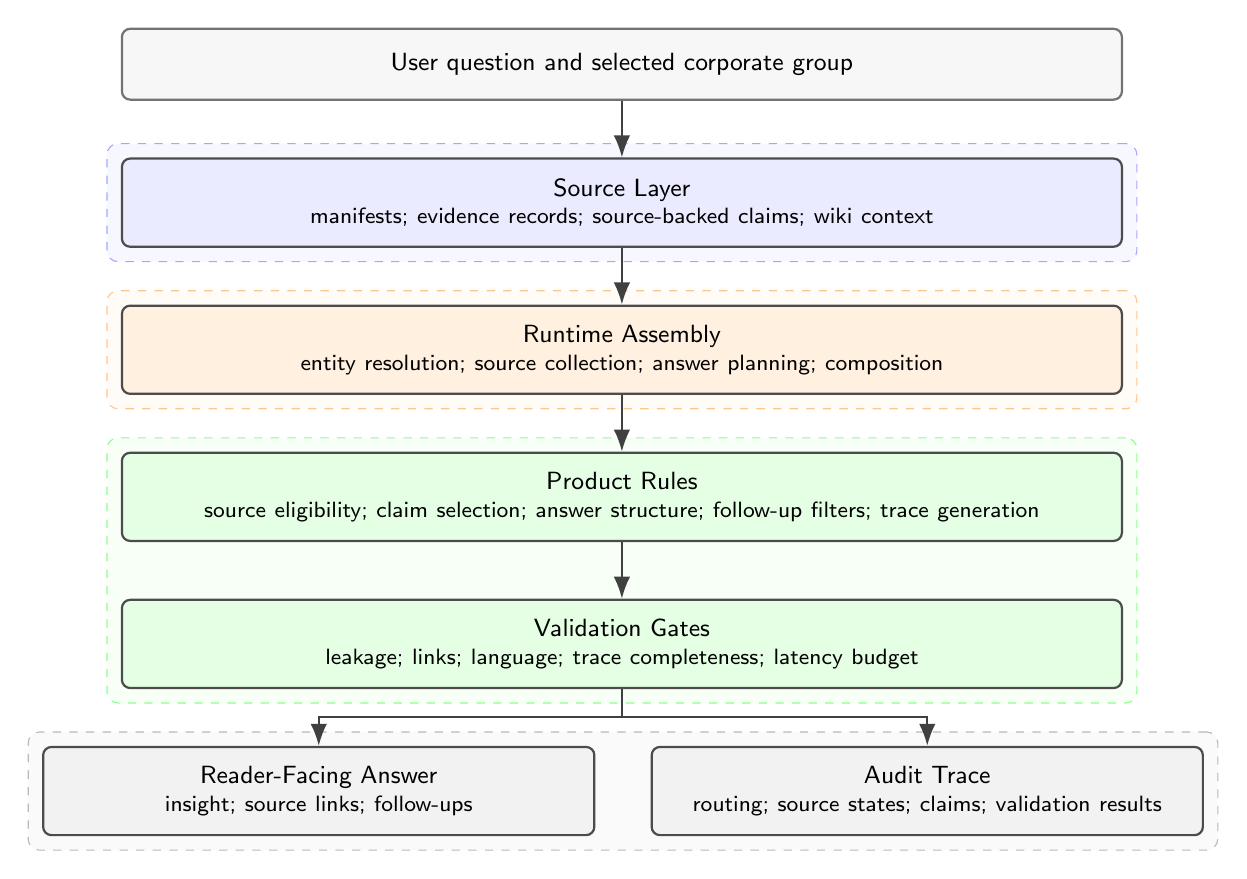
\begin{tikzpicture}[
    font=\small\sffamily,
    node distance=0.72cm,
    layer/.style={
        rectangle, rounded corners=3pt,
        draw=black!70, thick,
        minimum width=12.7cm, text width=12.4cm, minimum height=1.12cm,
        align=center,
        font=\small\sffamily
    },
    source/.style={layer, fill=blue!8},
    runtime/.style={layer, fill=orange!12},
    control/.style={layer, fill=green!10},
    output/.style={
        rectangle, rounded corners=3pt,
        draw=black!70, thick,
        fill=gray!10,
        minimum width=7.0cm, text width=6.75cm, minimum height=1.12cm,
        align=center,
        font=\small\sffamily
    },
    inputbox/.style={
        rectangle, rounded corners=3pt,
        draw=black!55, thick,
        fill=gray!6,
        minimum width=12.7cm, text width=12.4cm, minimum height=0.9cm,
        align=center,
        font=\small\sffamily
    },
    flow/.style={-{Latex[length=2.8mm]}, thick, draw=black!75},
    sideflow/.style={-{Latex[length=2.4mm]}, thick, draw=black!55, dashed},
    grouplabel/.style={font=\small\sffamily, text=black!55}
]

% ============ Main vertical architecture ============
\node[inputbox] (input) {User question and selected corporate group};

\node[source, below=of input] (source) {
    Source Layer\\[-1pt]
    \footnotesize manifests; evidence records; source-backed claims; wiki context
};

\node[runtime, below=of source] (runtime) {
    Runtime Assembly\\[-1pt]
    \footnotesize entity resolution; source collection; answer planning; composition
};

\node[control, below=of runtime] (boundary) {
    Product Rules\\[-1pt]
    \footnotesize source eligibility; claim selection; answer structure; follow-up filters; trace generation
};

\node[control, below=of boundary] (control) {
    Validation Gates\\[-1pt]
    \footnotesize leakage; links; language; trace completeness; latency budget
};

\node[output, below=of control, xshift=-3.85cm] (answer) {
    Reader-Facing Answer\\[-1pt]
    \footnotesize insight; source links; follow-ups
};
\node[output, right=0.7cm of answer] (trace) {
    Audit Trace\\[-1pt]
    \footnotesize routing; source states; claims; validation results
};

% ============ Flow ============
\draw[flow] (input) -- (source);
\draw[flow] (source) -- (runtime);
\draw[flow] (runtime) -- (boundary);
\draw[flow] (boundary) -- (control);
\draw[flow] (control.south) -- ++(0,-0.35) -| (answer.north);
\draw[flow] (control.south) -- ++(0,-0.35) -| (trace.north);

% ============ Background grouping ============
\begin{scope}[on background layer]
    \node[fit=(source), draw=blue!35, dashed, rounded corners, inner sep=5pt, fill=blue!3] {};
    \node[fit=(runtime), draw=orange!45, dashed, rounded corners, inner sep=5pt, fill=orange!3] {};
    \node[fit=(boundary)(control), draw=green!45, dashed, rounded corners, inner sep=5pt, fill=green!3] {};
    \node[fit=(answer)(trace), draw=gray!55, dashed, rounded corners, inner sep=5pt, fill=gray!4] {};
\end{scope}

\end{tikzpicture}
\end{document}
